\documentclass[english]{article}
\usepackage[utf8]{inputenc}
\usepackage[T1]{fontenc}
\usepackage[english]{babel}

\usepackage{graphicx}
\usepackage{hyperref}
\usepackage{nameref}
\usepackage{textcomp}
\usepackage{gensymb}
\newcommand{\hsp}{\hspace{20pt}}
\newcommand{\HRule}{\rule{\linewidth}{0.5mm}} 
\usepackage{float}
\usepackage{geometry}
\usepackage{ccaption}
\usepackage{amsmath}
\usepackage{amssymb}
\usepackage{textcomp}
\usepackage{mathabx}
\usepackage{stmaryrd}
\usepackage{verbatim}
\newcommand{\etal}{\textit{et al}., }

%\geometry{top=3cm, bottom=3cm, left=2cm, right=2cm}


\begin{document}


%%%%%%%%%%%%%%%%%
% PAGE DE GARDE %
%%%%%%%%%%%%%%%%%

\title{Global pyramidal analysis of images with a deeply supervised U-Net architecture}

\author{
Damien Djomby \and Tristan Michel \and Michele BONA \and Enzo Masson \and Clémence Gaillotte \\
Ecole de Technologie Supérieur
}
\date{Décembre 2021}

\maketitle
\normalsize


\begin{abstract}
This paper presents SubUNet, a model architecture for medical image segmentation (MRIs). Our model is inspired by the UNet architecture and adds the Pyramid Pooling Module (PPM) of the PSPNet architecture. This module serves mainly to add a global observation of our image by increasing the receptive field of the model. This helps to detect the various parts of the heart by their shape and according to the organs surrounding it. Thus, by combining the precision of Unet for the details of the images and the PPM, we can detect the left and right ventricles and the myocardial on MRIs of hearts with better precision than a basic UNet implementation.
\end{abstract}


\section{Introduction}  

\subsection{Problem}
\paragraph{}
In recent decades, magnetic resonance imaging (MRI) has become an essential medical imaging technique for studying the human heart. However, due to the characteristics of cardiac MRIs and the large variability of images between patients, the problem of automatic identification of the different parts of the heart in MRIs has arisen and is still under intense study.
\paragraph{}
On the other hand, research on image processing by neural networks is constantly evolving, and the subject of automatic segmentation of MRIs is progressing with it. Thus one may wonder how to automatically identify the left and right ventricles and the myocardium on human heart MRIs.
\paragraph{}
This type of segmentation requires medical knowledge of the human heart, and developing a neural network that does it automatically would help analyze MRIs and speed up doctors' diagnoses.

\subsection{Contributions}
\paragraph{}
As we will see in the \nameref{method} section, we were inspired by the most efficient and used neural networks, particularly U-Net. After implementing them and creating our model, we noticed that we had slightly better segmentation than U-Net, and very satisfactory accuracy for segmenting the right ventricle, which generally is the hardest challenge on this dataset.


\section{State of the art}
\paragraph{}
Machine learning is now at the center of many medical imaging research topics because of the significant advances it could bring to the medical community. Therefore, this is the subject of many machine learning challenges. Allowing researchers to propose increasingly efficient models for these challenges.

\subsection{Medical imaging segmentation methods}
\paragraph{}
Many models are responding to the problems of medical imaging segmentation, and we will focus on a few models and cost functions that have stood out from the others.

%U-net
\subsubsection{U-Net}
\paragraph{}
This is the case of the U-Net network known for its U-shaped architecture. It is a fully convolutional network that is based on a fully connected network (FCN).

\paragraph{}
U-Net was created by \emph{Olaf Ronneberger, Philipp Fischer and Thomas Brox} in 2015 as part of their participation and victory in the ISBI challenge (segmentation challenge for medical imaging) in November 2015. The score of their model outperformed other models' scores by more than 10\%. The U-net network was presented more explicitly in their paper \emph{U-Net: Convolutional Networks for Biomedical Image Segmentation} \cite{UNet}. Since then, the network has been taken over and slightly modified by many teams as part of segmentation for medical imaging.

\paragraph{}
In 2018, the U-Net++ \cite{U-Net++} network retained the principle of an encoding sub-network and then a decoding sub-network. One of the main modifications is the link between these two sub-networks with Skip connections as well as the use of deep supervision

\paragraph{}
Finally, the GA-Unet \cite{GA-UNet} network was released in 2021. The model uses the convolutional neural network VGG16 as an encoder of the U-Net network. The pooling layers present in U-Net are replaced by upsampling operations.

\subsubsection{PSPNet}
\paragraph{}
The PSPNet network \cite{PSPNet} is a model created as part of the ImageNet Scene Parsing Challenge in 2016. This network is not specially designed for medical imaging but obtains very efficient segmentation results regarding global information.
\paragraph{}
This network comprises an encoder-decoder architecture and a pyramid pooling module (PPM). This module allows for a global context to the image before making a local prediction. This is an improvement over ResNet \cite{ResNet}, a model that has encountered difficulties in capturing the global context of an image despite a very large receptive input field.

\subsection{Cost functions}
\paragraph{}
There are many cost functions, but some have better demonstrated their effectiveness in medical imaging segmentation problems. There is cross-entropy which is very often used. This cost function operates at the pixel level and is the basis for many other cost functions. But alone, this function does not help to reduce errors using global information.
\paragraph{}
A cost function regularly used in medical imaging segmentation is Dice loss. This function makes it possible to calculate the similarity between two images and allows a better definition of the contours.
\paragraph{}
Finally, there is the Focal Loss introduced within the framework of the detection of dense objects \cite{Focal-Loss}. This variation of Cross-entropy allows putting more weight on examples that have been difficult to classify. This function has the specificity to work very well even if the classes are not balanced. It generally has a good impact on the speed of convergence.


\section{Method}
\label{method}

\subsection{Training data}
\paragraph{}
Our training data is 1208 different heart MRIs from less than a hundred patients (and 90 validation images). The images show a heart in different cross-sections, all in shades of gray and 256x256 in size.
The only pre-processing we applied was to balance the grayscale histogram of the images.

\subsection{Data augmentation}
\paragraph{}
The human body is complex and has vast organ placement and size variability.
This is particularly noticeable when trying to segment images of human hearts to detect the different parts. Due to the size of our dataset and to avoid over-fitting, we have implemented a Data Augmentation that remains consistent with the possibilities we may encounter with actual patients.
For this, it was necessary to consider different malformations that may affect patients. Thus, we have about ten possible transformations, each with a probability of 0.2 to be applied. This high value allows us to train our model on very varied data.
The possible transformations are:

\begin{list}{\textbullet}{}
    \item a vertical flip (mirror on the horizontal axis)
    \item a horizontal flip mirror
    \item a rotation with an angle ranging from -30° to 30° chosen from a linear distribution
    \item a crop (zoom), the size of the subframe is between 50\% and 100\% of the original frame's size, the position of the subframe depends on a randomly chosen edge
    \item a padding (adding a black margin)
    \item a z shift
    \item a brightness shift
    \item a Gaussian blur (which was very useful to us)
    \item a self-contrast
    \item a sharpness change (with a value between 0 and 2)
\end{list}


\subsection{Choice of model}
\paragraph{}
Empirically, research has amply proven that the UNet framework is one of the most efficient model for medical imaging segmentation.
To keep the input size of our images after applying the model, we chose to add padding for the convolutions instead of making a mirror padding as presented by Ronneberger \etal\cite{UNet}.
This avoids the zoom present among the feature maps we find in UNet. We did not want to lose information as even edge information could impact the prediction.
\paragraph{}
Following our experiments, we had better results with the UNet and PSPNet models (probably thanks to the Pyramid Pooling Module). These results are consistent with the fact UNet is designed for medical segmentation.
In addition, the PSPNet's PPM module allows us to have a more global context in our detection and thus try to identify shapes surrounding the heart (for example, locate the heart in relation to the lungs).
We have added Deeply-Supervised modules in the UNet decoder to control learning in the right direction. Unfortunately, their effectiveness is not conclusive, as we will present in the section \ref{robustness}.
\paragraph{}By combining UNet's encoder and decoder with PSPNet's PPM, we should have a model capable of performing precise segmentation (due to UNet's skip connections).
Thanks to a global observation of our image from the PPM, we should be able to detect the different parts of the heart by their shape and according to the organs surrounding it.
Moreover, according to state of the art and our experiments, we used Average Poolings instead of Max Poolings in the UNet encoder as we witnessed better results when combined with the PPM module. The section \ref{robustness} also presents the advantages of Avg Pooling.
This model, presented in figure \ref{model}, allows segmentation with environment consistency by taking advantage of UNet and PPM.


\begin{figure}[!t]
    \centering
    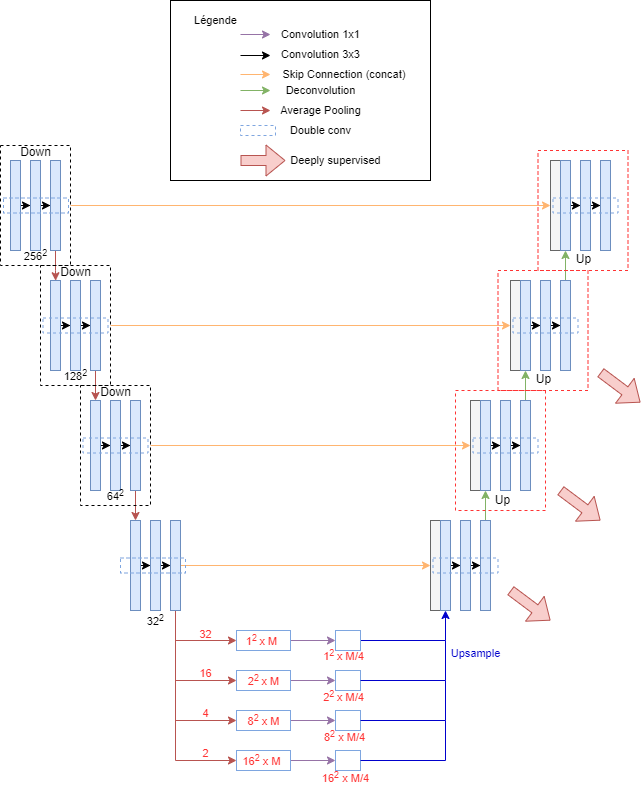
\includegraphics[scale=0.45]{img/SubUnetAvecPPM.png}
    \caption{Architecture of our model, based on a UNet encoder and decoder with Average pooling and de-convolution, and a pyramidal pooling module.}
    \label{model}
\end{figure}

\subsection{Network training}
\label{training}

\paragraph{}We trained our model with a batch size of 56 images. Our research has shown that a large number of images per batch gives better results. For the update of our parameters, we have chosen to use the policy of `poly' learning rate where the learning rate of the epoch is equal to the starting learning rate of \(3, 15\times 10^{-4}\) multiplied by $(1-\frac{iter}{max_iter})^{power}$. For the power value, we took the same value as the one presented in the PSPNet paper, ie \(0.9\). Regarding the cost function, we used a combination of the Dice coefficient and Focal loss \(loss(X,Y) = \alpha \cdot FocalLoss_{\gamma}(X,Y)+(1-\alpha) \cdot DiceLoss(X,Y)\), with \(\alpha=0.233\) and \(\gamma=1.977\).
\paragraph{}Inspired by Ye \etal\cite{multidepth_fusion}, our deeply supervised branches are a succession of 2D transposed Convolution allowing us to go back to the original size of the input image. We then calculate the error of each prediction (main and supervised branches) compared to the ground truth and sum these errors. The backpropagation is calculated from this result and propagated to the model.





\section{Results}

\subsection{Results on the challenge}
\paragraph{Comparison with other models}
\label{comp:models}
We performed a grid search during our preliminary research to determine which models and cost functions were the most promising for the segmentation challenge. We have implemented the SegNet, PSPNet (with a simple encoder instead of ResNet), and UNet models, as well as an adaptation of VGG allowing segmentation. We also studied different cost functions whose research and results will be presented in the \nameref{loss_ablation} section. Table \ref{tab:baseline} presents the results obtained for this gridsearch. Unsurprisingly, UNet appeared to be the most successful on our dataset. However, PSPNet also gave good results even though the latter was implemented with a much simpler encoder and decoder than the one described by Zhao \etal\cite{PSPNet}. This is why we came up with the idea of using the Pyramid Pooling Module within a UNet.

\begin{table}[h]
    \centering
    \footnotesize
    \begin{tabular}{l l c c c}
        \hline
        Model & Cost Function & Mean IoU(\%) & Mean Dice(\%) & Mean Soft Dice(\%)\\
        \hline
        \hline
        VGG & focal tversky loss + focal loss & 65,92 & 77,81 & 19,55\\
        SegNet & jaccard loss + focal loss & 77,18 & 86,33 & 19,37\\
        \textit{PSPNet} & ce loss & \textit{79,44} & \textit{87,86} & \textit{20,35}\\
        \textbf{UNet} & jaccard loss & \textbf{85,52} & \textbf{92,01} & \textbf{92,29}\\
        \hline
    \end{tabular}
    \caption{Best results obtained after the grid search for each model, specifying the cost function that gave these results.}
    \label{tab:baseline}
\end{table}

% grid search
\paragraph{Convergence rate}
As shown in figure \ref{fig:convergence}, SubUNet converges faster than UNet when trained with our deeply supervised module. Yet, the section \ref{robustness} will show that we obtained better results without this module but with a lower convergence speed.

\begin{figure}[h]
    \centering
    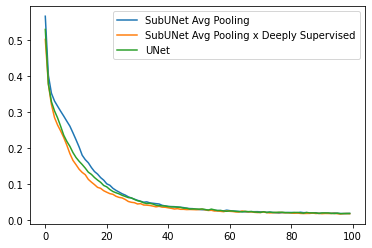
\includegraphics[scale=0.8]{img/convergence.png}
    \caption{Comparison of convergence of the cost function on the training dataset for our baseline and our model with and without deeply supervised module.}
    \label{fig:convergence}
\end{figure}


\paragraph{Visual improvements}
As shown in figure \ref{fig:baseline}, our model allows a better prediction of the right ventricle, which is, in our opinion, the hardest class to predict. Since it can also be the preponderant class on some images, the latter can considerably lower the score of a model with difficulty generalizing. We notice that UNet has more difficulty in predicting the right ventricle. This prediction problem on the right ventricle with UNet is a problem we identified from the start of the challenge and is the main point we have tried to solve. Thus, at the end of our research, the proposed model generally has a prediction closer to the ground truth for this ventricle.

\begin{figure}[h]
    \centering
    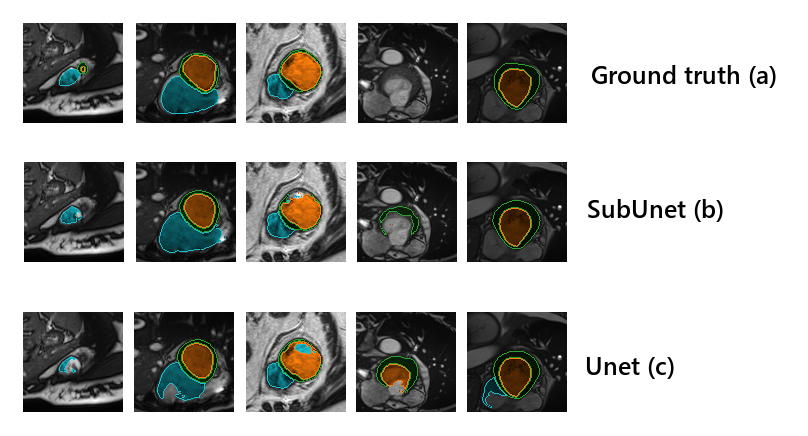
\includegraphics[scale=1.75]{img/comparaison.png}
    \caption{Visual improvement on the challenge dataset of our model (b) compared to our baseline (c). This figure shows the left ventricle in \textit{orange}, the myocardium of the left ventricle in \textit{green}, and the right ventricle in \textit{blue}. Both models, SubUNet and our baseline were trained under the same conditions.}
    \label{fig:baseline}
\end{figure}




\subsection{Robustness study of our method}
\label{robustness}

\subsubsection{Ablation study of the model}
\paragraph{}
To study the performance of our model, compared to our baseline, we performed various model training with different configurations. Those include the type of pooling used and the use or not of our deeply supervised module. As listed in the table \ref{tab:ablation:model}, average pooling works better than max pooling, which matches the results obtained by Zhao \etal\cite{PSPNet}. We also noticed that our deeply supervised module did not give such good results, which can be explained by a bad implementation or that we sent a too strong gradient on the supervised branches, thus lowering the precision in the main branch.

\begin{table}[H]
    \footnotesize
    \centering
    \begin{tabular}{ l c c c }
        \hline
        Method & Mean IoU(\%) & Mean Dice(\%) & Mean Soft Dice(\%) \\
        \hline\hline
        %FCN \cite{long2015fully} & 29.39 & 71.32 \\
        PSPNet & 79,62 & 88,20 & 90,50 \\
        UNet & 84,77 & 91,49 & 93,10 \\
        SubUNet MP & 85,10 & 91,75 & 93,41 \\
        SubUNet MP x Deeply Supervised & 85,13 & 91,78 & 93,31 \\
        SubUNet AP x Deeply Supervised & 85,50 & 92,02 & 93,58 \\
        \textbf{SubUNet AP} & \textbf{85,63} & \textbf{92,06} & \textbf{93,65} \\
        \hline
    \end{tabular}
    \caption{Study of our model according to different parameters. `MP' and `AP' stand for `Max Pooling' and `Average Pooling' respectively, and `DP' is for our deeply supervised module. Our results were obtained on the validation dataset after training with our best hyperparameters (detailed in section \ref{hyperparameters}) and with data augmentation over 400 epochs.}
    \label{tab:ablation:model}
\end{table}

\subsubsection{Ablation study of the hybrid cost function}
\label{loss_ablation}
\paragraph{}
As described in the \ref{comp:models} section, we performed a gridsearch to explore which cost functions and which baseline models performed best. Therefore, we determined that for this challenge, the couple \(Dice Loss + Focal Loss\) allowed a noticeable improvement in performance. The main idea was to see if combining a set cost function (which compares the prediction and the ground truth as sets) and a pixel-wise cost function would give better results. This gridsearch showed that a combination usually gives slightly better results. The table \ref{tab:ablation:loss} presents the results obtained by ablation on the cost function \(Dice + Focal\) with our SubUNet model.

\begin{table}[H]
    \footnotesize
    \centering
    \begin{tabular}{ l c c c }
        \hline
        Method & Mean IoU(\%) & Mean Dice(\%) & Mean Soft Dice(\%) \\
        \hline\hline
        Focal loss & 81,29 & 89,17 & 90,39 \\
        Dice loss & 85,59 & 91,78 & 93,32 \\
        \textbf{Dice loss + Focal loss} & \textbf{85,75} & \textbf{92,08} & \textbf{93,68} \\
        \hline
    \end{tabular}
    \caption{Ablation study of the cost functions used. Our results were obtained on our SubUnet model with our best hyperparameters and data augmentation over 200 epochs. The combination \(Dice + Focal\) was obtained with a \(\alpha=0.5\). The \ref{hyperparameters} section presents the optimal value we obtained for this parameter.}
    \label{tab:ablation:loss}
\end{table}

\subsubsection{Hyperparameters}
\label{hyperparameters}
\paragraph{}
To determine the hyperparameters of our model, we performed a random search on the following parameters: the batch size, the \(\alpha\) and the \(\gamma\) of our cost function presented in the \nameref {training} section as well as the learning rate. For our random search, we performed 200 training of 400 epochs each. The learning rate was drawn according to a normal distribution and then brought to the power of 5 to obtain small values. Let \(r\) be a random value between 0 and 1, \(lr = r^5\). Table \ref{tab:comp_params} presents the results of this search and the best parameters we obtained and used for training our models. Nevertheless, it would seem that even larger batches could have given better results. Still, we found ourselves faced with a technological problem: beyond 60 images per batch, we were reaching the RAM limit of our graphics cards (our models were trained on Nvidia A100 cards, with 40GB of graphical RAM, and the entire dataset was loaded on RAM to reduce the training duration).

\begin{table}[H]
    \footnotesize
    \centering
    \begin{tabular}{c c c c c c c}
        \hline
        Batch & \(\alpha\) & \(\gamma\) & lr & mean iou(\%) & mean dice(\%) & mean soft dice(\%)\\
        \hline
        \hline
        \([1;100]\) & \([0;1]\) & \([0;4]\) & \([0;1]\) \\
        \hline
        63 & 0,054 & 1,351 & \(1,52\times 10^{-2}\) & 87,53 & 93,24 & 94,70\\
        67 & 0,461 & 2,676 & \(7,15\times 10^{-4}\) & 88,12 & 93,60 & 94,95\\
        62 & 0,879 & 3,604 & \(3,93\times 10^{-4}\) & 88,54 & 93,82 & 95,09\\
        73 & 0,490 & 1,737 & \(6,29\times 10^{-4}\) & 88,91 & 94,05 & 95,38\\
        \textbf{56} & \textbf{0,233} & \textbf{1,977} & \textbf{\(3,15\times 10^{-4}\)} & \textbf{89,35} & \textbf{94,28} & \textbf{95,47}\\
        \hline
    \end{tabular}
    \caption{This table presents the best results obtained during our random search. The top section presents the intervals used, and the last line of the bottom section presents our best settings.}
    \label{tab:comp_params}
\end{table}


\section{Conclusion}
\paragraph{}
Finally, our model is quite efficient for the medical imaging segmentation challenge. We've enhanced U-Net by adding PSPNet's Pyramid Pooling Module (PPM) system, which improved the model precision to detect the different classes but, most importantly, the right ventricle, representing a real challenge by itself. Due to the size of the dataset, the data augmentation process we implemented surely helped the model to generalize and complement the precision of the model.
\paragraph{}
For each parameter, all our data is stored with their associated measurements. It would therefore be possible to statistically study the impact of hyperparameters on performance to find the best values for the hyperparameters experimentally.


\newpage

\bibliographystyle{plain} % We choose the "plain" reference style
\bibliography{refs} % Entries are in the refs.bib file

\end{document}

